%
% teil3.tex -- Beispiel-File für Teil 3
%
% (c) 2020 Prof Dr Andreas Müller, Hochschule Rapperswil
%
% !TEX root = ../../buch.tex
% !TEX encoding = UTF-8
%
\section{Geostrophische Näherung / heutiger Ansatz
\label{geostrophisch:section:geoNäherung}}
\kopfrechts{Geostrophische Näherung}
\subsection{Geostrophische Näherung}
Das Gleichgewicht zwischen der Druckgradientkraft und der Coriolis-Kraft wird in der geostrophischen Näherung durch folgende Beziehung dargestellt:
\index{Coriolis-Kraft}%
\begin{equation}
f\, (\vec{k} \times \vec{v}_g) 
+
\frac{1}{\rho} \nabla p
=
0.
\label{geostrophisch:equation5}
\end{equation}
Von der geostrophischen Näherung spricht man also, wenn man annimmt, dass sich die Druckgradientkraft und Coriolis-Kraft im Gleichgewicht befinden und alle anderen Kräfte vernachlässigt werden können. In diesem Fall wirken beide Kräfte gleich stark, aber in entgegengesetzte Richtungen, sodass kein weiterer Beschleunigungseffekt auf die Luftmasse wirkt und sie parallel zu den Isobaren strömt. Es entsteht der sogenannte geostrophische Wind.

\vspace{1em}

Da die genaue Masse eines Luftpakets meist nicht bekannt ist, betrachtet man beide Kräfte pro Masseneinheit. Entsprechend handelt es sich bei den dargestellten Gleichungen um spezifische Kräfte, also Beschleunigungen.

\vspace{1em}

Mathematisch entspricht das dem Gleichgewicht zwischen der Druckgradientkraft nach Gleichung \eqref{geostrophisch:equation4} und der Coriolis-Kraft nach Gleichung \eqref{geostrophisch:equation2}.

\subsection{Heutiger Ansatz}

Der heutige Ansatz in der numerischen Wettervorhersage entspricht im Wesentlichen der Vision von Lewis Fry Richardson, allerdings mit den Möglichkeiten moderner Hochleistungsrechner.
\index{Hochleistungsrechner}%

\begin{itemize}
    \item Die Atmosphäre wird in ein dreidimensionales Gitter unterteilt, das sowohl horizontale als auch vertikale Auflösung umfasst.
    \item Auf jedem Gitterpunkt werden die fundamentalen Erhaltungsgleichungen (insbesondere die Navier-Stokes-Gleichungen) gelöst, um die Entwicklung von Wind, Temperatur, Luftdruck und weiteren Grössen zu berechnen.
    \item Dabei kommen umfangreiche Echtzeitdaten zum Einsatz, die durch Satelliten, Bojen, Flugzeuge und Wetterstationen bereitgestellt werden.
\index{Echtzeitdaten}%
\index{Satelliten}%
\index{Boje}%
\index{Flugzeug}%
\index{Wetterstation}%
    \item Hochleistungsrechner (Supercomputer) berechnen die Entwicklung der atmosphärischen Zustandsgrössen iterativ in kleinen Zeitschritten – diese bildet die Grundlage der numerischen Wettervorhersage (Numerical Weather Prediction, NWP).
\index{Supercomputer}%
\index{NWP}%
\index{numerical weather prediction}%
\index{numerische Wettervorhersage}%
\end{itemize}

Die Gleichung zur Beschreibung der zeitlichen Änderung des Wasserdampfgehalts (die sogenannte ``7.~Gleichung'') wurde in diesem Zusammenhang bewusst ausgelassen, unter anderem weil die Atmosphäre in früheren Modellen als deutlich trockener angenommen wurde als heute.
\index{Wasserdampfgehalt}%

\subsection{Die siebte Gleichung}

In der klassischen Formulierung der atmosphärischen Grundgleichungen besteht das System aus sieben Gleichungen:  
\begin{itemize}
    \item drei Bewegungsgleichungen (Navier-Stokes in $x$-, $y$- und $z$-Richtung),
    \item die Kontinuitätsgleichung (Massenerhaltung),
    \item die Energiegleichung,
    \item die Zustandsgleichung (ideales Gas),
    \item und die Feuchtegleichung.
\end{itemize}

Letztere wird daher als \emph{siebte Gleichung} bezeichnet. Sie beschreibt die zeitliche Änderung des spezifischen Wasserdampfgehalts $q_v$ in der Luft. Dabei handelt es sich um eine Erhaltungsgleichung, die sowohl den Transport von Feuchtigkeit als auch Quellen und Senken wie Kondensation, Verdunstung oder Niederschlag berücksichtigt.  

In ihrer allgemeinen Form lautet sie:

\begin{equation}
\frac{\partial q_v}{\partial t} + \vec{v} \cdot \nabla q_v = S_q
\tag{19.10}
\end{equation}
mit:  
\begin{itemize}
    \item $q_v$: spezifischer Wasserdampfgehalt in kg Wasserdampf pro kg feuchter Luft $[\mathrm{kg/kg}]$
    \item $\vec{v}$: Windvektor (Strömungsgeschwindigkeit der Luft)
    \item $S_q$: Quell- und Senkenterm (z. B. durch Phasenübergänge wie Kondensation oder Verdunstung)
\index{Phasenübergang}%
\end{itemize}

Diese Gleichung ist von zentraler Bedeutung für die Beschreibung der Feuchteverteilung in der Atmosphäre und damit für die Modellierung von Wolkenbildung, Niederschlagsprozessen und die Vorhersage des Wetters.
\index{Wokenbildung}%
\index{Niederschlag}%


\subsection{Moderne Umsetzung nach Richardson} 

Aufbauend auf den theoretischen Grundlagen und der Methodik von Richardson wurde ein eigener Ansatz entwickelt, der mithilfe heutiger Rechenleistung die Berechnung des geostrophischen Windes automatisiert.
Hierfür wurde ein Python-Programm erstellt, das auf Basis realer atmosphärischer Druckdaten die horizontalen Druckgradienten ermittelt und unter Berücksichtigung der Coriolis-Kraft den geostrophischen Wind berechnet.
\index{Python}%
Das Programm visualisiert die Resultate in Form von Vektorfeldern, sodass sowohl Geschwindigkeit als auch Richtung des Windes anschaulich dargestellt werden.
\index{Vektorfeld}%
\index{Geschwindigkeit}%

Dieser moderne Ansatz verbindet die historischen Ideen Richardsons mit den heutigen Möglichkeiten der Datenverarbeitung und Visualisierung, wodurch eine präzisere und deutlich schnellere Analyse atmosphärischer Strömungen möglich wird.

Die Luftdruckdaten beziehen wir von einer Internetseite namens OpenWeatherMap.
\index{Luftdruckdaten}%
\index{OpenWeatherMap}%
Als erstes haben wir eine Liste erstellt mit den Städten und dazugehörigen Koordinaten, der Orte die wir auf der Karte gerne angezeigt haben möchten.
Anschliessend werden von allen Ortschaften die Druckdaten von der Internetseite gelesen.
Danach erstellen wir ein Gitter mit den Koordinaten der Ortschaften, indem wir zuerst die Längen- und Breitengrade vom kleinsten bis zum grössten Wert mit konstanten Schritten aufteilen.
Anschliessend interpolieren wir für jeden Punkt im Gitter den lokalen Luftdruck.
Druckgradienten müssen wir in \(x\)- sowie \(y\)-Richtung einzeln berechnen.
Doch dafür brauchen wir zuerst noch die Längen- und Breitengradabstände ($dx$, $dy$).
Der Längengradabstand berechnet sich wie folgt
\begin{equation}
	\frac{2 \pi R}{360^\circ} \cos(\varphi), 
\end{equation}
wobei das $R$ für den Erdradius ($\approx\SI{6371}{\kilo\meter}$) steht. 
Die Breitengrade sind Parallelkreise und deren Umfang nimmt vom Äquator zu den Polen ab.
Deren Abstand ist konstant $\approx\SI{111}{\kilo\meter}$.
Aus diesen Werten können wir nun den Druckgradienten berechnen, indem wir die Druckänderung zwischen benachbarten Punkten durch die Abstände teilen.
Jetzt haben wir schon so gut wie alles, um den geostrophischen Wind zu berechnen, wir brauchen nur noch den Coriolis-Parameter $f$.
Diesen berechnen wir wie in~\ref{geostrophisch:subsection:coriolis} schon gezeigt. 
Zur Farbgebung berechnen wir noch die Windgeschwindigkeit an jedem Punkt. 
Alles was danach im Code kommt, ist nur noch zur Darstellung der Daten und auf diese muss jetzt nicht genauer eingegangen werden.

Nachfolgend unser Python Code zum berechnen des geostrophischen Windes: 
\lstinputlisting[style=pycode]{papers/geostrophisch/PythonCode/geostrophischeNaeherungLiveData.py}

\begin{figure}
	\centering
	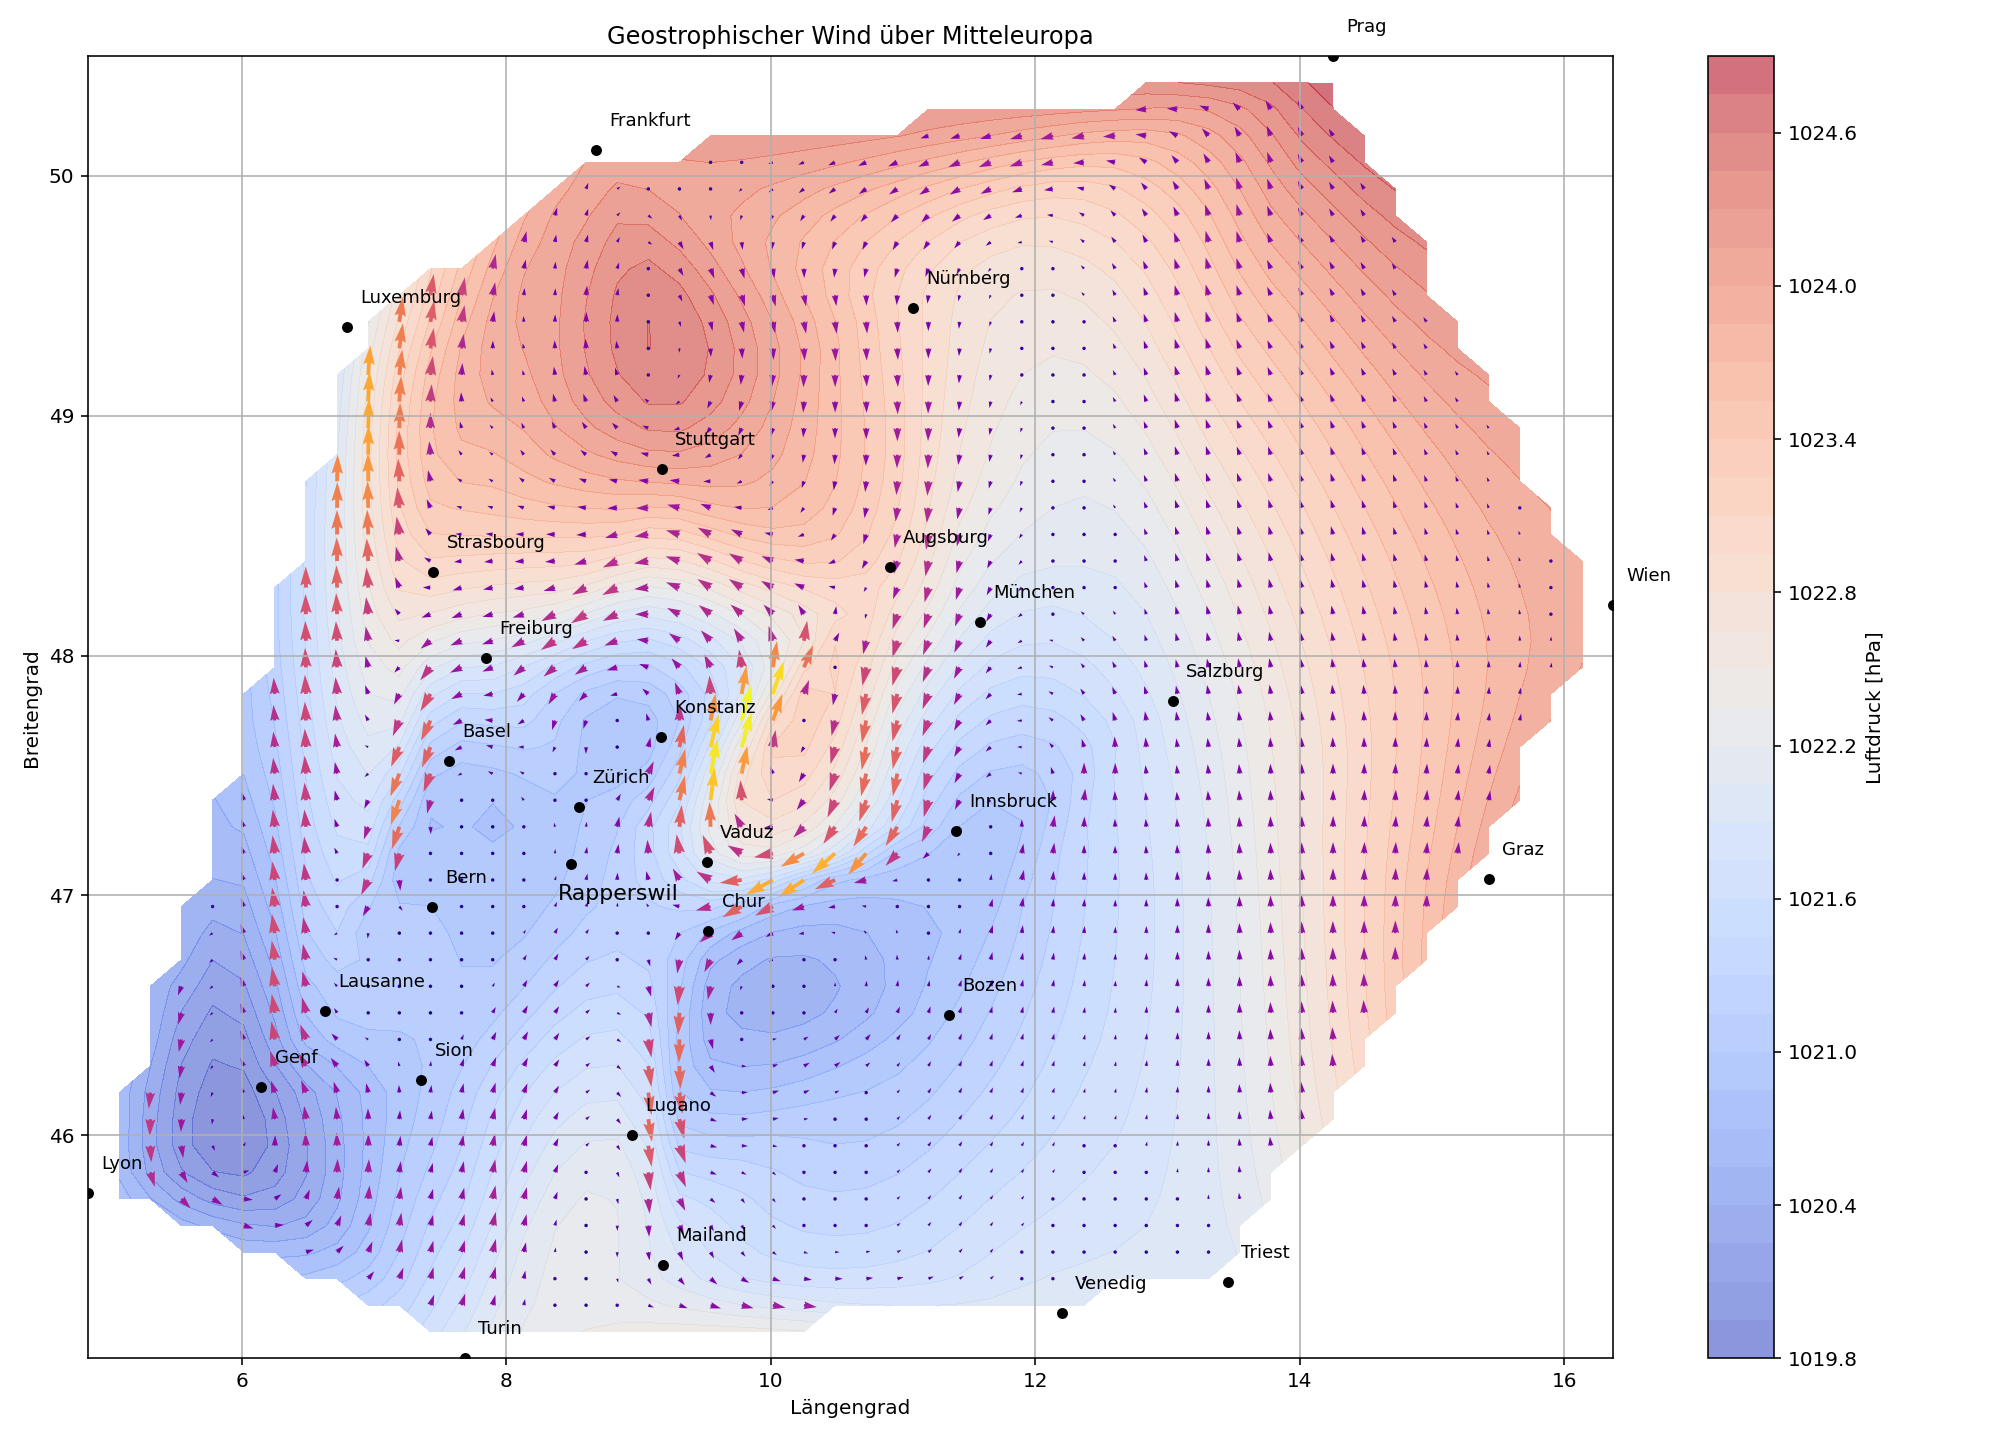
\includegraphics[width=\linewidth]{Python28042025.png}
	\caption{Diese Abbildung zeigt den geostrophischen Wind berechnet durch das Python Programm.
	Dieses Bild wurde am 28. April 2025 erstellt.
	Man sieht sehr gut, wo Tief- und Hochdruckgebiete liegen und wie der Wind parallel um diese weht.}
	\label{bild:28042025}
\end{figure}

\begin{figure}
	\centering
	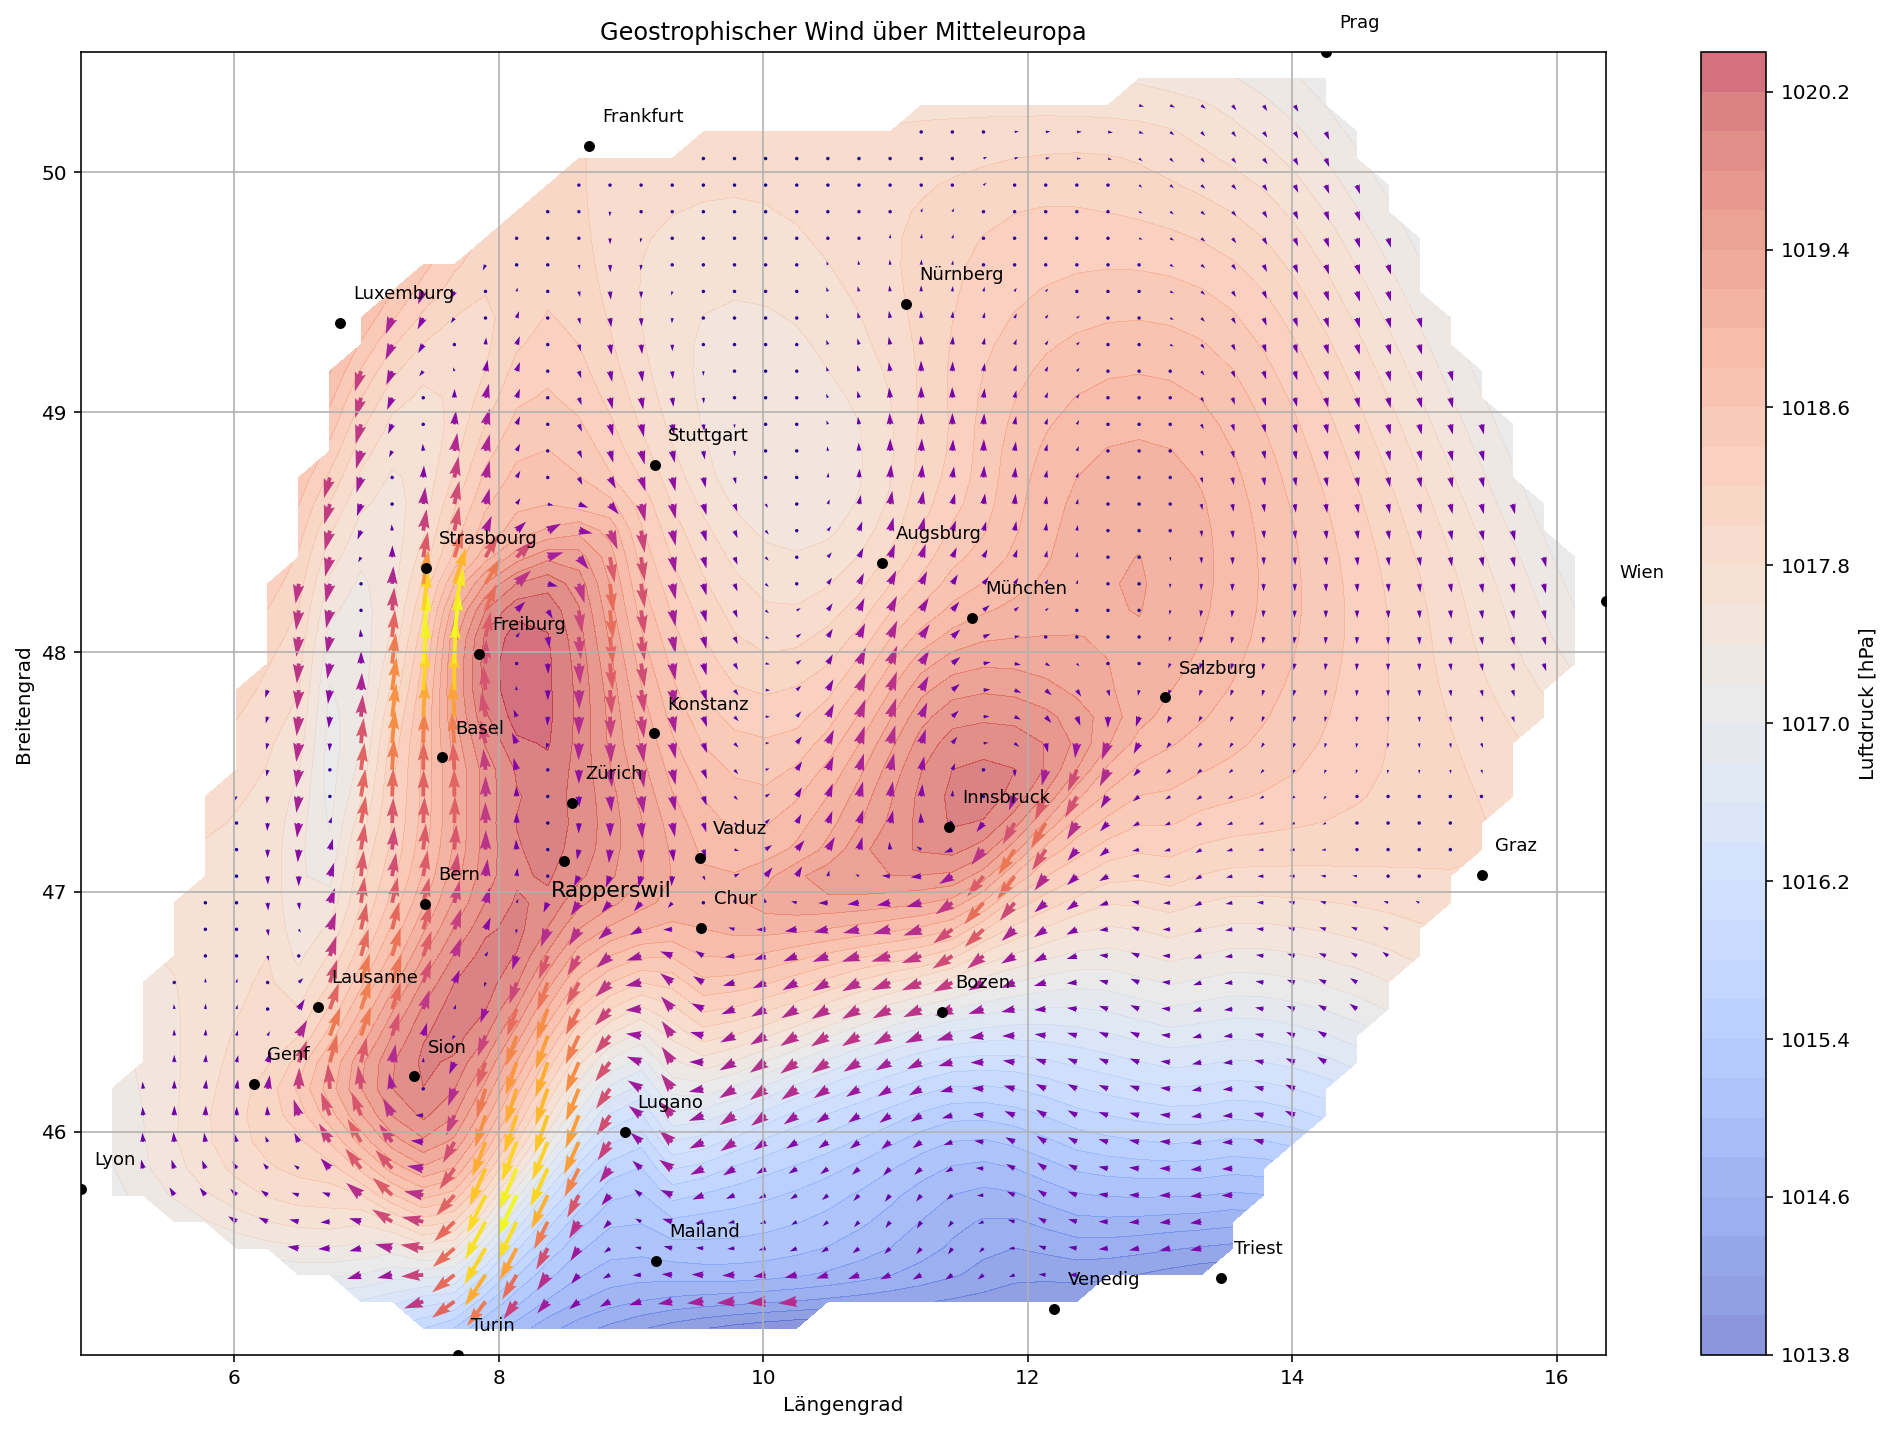
\includegraphics[width=\textwidth]{Python15082025.png}
	\caption{Eine Weitere Abbildung des geostrophischen Windes.
	Diese wurde am 15. August 2025 erstellt.
	}
	\label{bild:15082025}
\end{figure}


